\documentclass[twoside,a4paper,11pt,answers,addpoints]{exam}


\title{XX 1}
\date{}
\author{Juliette Fenogli}


\usepackage{siunitx}
\usepackage{mystyles}
\usepackage[export]{adjustbox}
\usepackage{mathpazo}
\usepackage{booktabs}
\usepackage{framed}
\usepackage{listings}
\usepackage{mhchem}



\lstset
{upquote=true,
columns=flexible,
    basicstyle=\small\tt\hbox{}, 
	basicstyle=\ttfamily,
	language=Python,
    framesep=\fboxsep,
    framerule=\fboxrule,
    xleftmargin=\dimexpr\fboxsep+\fboxrule,
    xrightmargin=\dimexpr\fboxsep+\fboxrule,
	commentstyle=\color{gray},
	frame=single,
	rulecolor=\color{green!5},
	backgroundcolor=\color{gray!5},
	breaklines,
	numbers=left, 
	numbersep=5pt,  
	numberstyle=\scriptsize \ttfamily\color{gray},
	breakindent=1.5em,
	literate={Δ}{{$\mathtt{\Delta}$}}1 {‡}{{$\mathtt{\ddagger}$}}1
  {á}{{\'a}}1 {é}{{\'e}}1 {í}{{\'i}}1 {ó}{{\'o}}1 {ú}{{\'u}}1
  {Á}{{\'A}}1 {É}{{\'E}}1 {Í}{{\'I}}1 {Ó}{{\'O}}1 {Ú}{{\'U}}1
  {à}{{\`a~}}1 {è}{{\`e}}1 {ì}{{\`i}}1 {ò}{{\`o}}1 {ù}{{\`u}}1
  {À}{{\`A~}}1 {È}{{\'E}}1 {Ì}{{\`I}}1 {Ò}{{\`O}}1 {Ù}{{\`U}}1
  {ä}{{\"a}}1 {ë}{{\"e}}1 {ï}{{\"i}}1 {ö}{{\"o}}1 {ü}{{\"u}}1
  {Ä}{{\"A}}1 {Ë}{{\"E}}1 {Ï}{{\"I}}1 {Ö}{{\"O}}1 {Ü}{{\"U}}1
  {â}{{\^a}}1 {ê}{{\^e}}1 {î}{{\^i}}1 {ô}{{\^o}}1 {û}{{\^u}}1
  {Â}{{\^A}}1 {Ê}{{\^E}}1 {Î}{{\^I}}1 {Ô}{{\^O}}1 {Û}{{\^U}}1
  {œ}{{\oe}}1 {Œ}{{\OE}}1 {æ}{{\ae}}1 {Æ}{{\AE}}1 {ß}{{\ss}}1
  {ç}{{\c c}}1 {Ç}{{\c C}}1 {ø}{{\o}}1 {å}{{\r a}}1 {Å}{{\r A}}1
  {€}{{\EUR}}1 {£}{{\pounds}}1 {×}{{$\times$}}1,       
}


\usepackage{adjustbox}
\usepackage{colortbl}
\usepackage{fontawesome}
\usepackage{todonotes}
\usepackage{listings} %codes python

%Columns Spacing
\newcolumntype{C}[1]{>{\centering\let\newline\\\arraybackslash\hspace{0pt}}m{#1}}
\newcolumntype{M}[1]{>{\centering\arraybackslash}m{#1}}


\newcounter{foo} %Counter questions

\begin{document}
%
\includepdf[pages = {1}]{page-garde.pdf}

\tito{Expériences autour des concepts de base d'électrochimie pour l'énergie}

\paragraph*{But} 
Lors de cette séance de TP, vous serez emmené à revisiter les concepts élémentaires des réactions rédox par une approche expérimentale. Avant toute chose, l'objectif est de se familiariser avec plusieurs concepts théoriques vus au Chp. 1 du cours sur les batteries.

\tableofcontents

\section{\'{E}chelle de potentiel électrochimique - \faClockO ~ \SI{30}{\minute}}

Vous cherchez à mettre en place une pile galvanique présentant les meilleures performances énergétiques. Pour cela, vous allez devoir classer des métaux en fonction de leur noblesse, notion expérimentale. Par définition, un métal est dit noble lorsqu'il résiste à la corrosion et à l'oxydation.

Lors de votre arrivée au laboratoire, votre travail sera contraint par le matériel disponible :
\begin{center}
\begin{tabular}{ccc}
Solides & Solutions à \SI{0.01}{\mole\per\liter} & Verrerie \\
\ce{Cu(s)} & \ce{Cu^{2+} (aq)} & Pipette Pasteur \\
\ce{Zn(s)} & \ce{Zn^{2+} (aq)} & \\
\ce{Al (s)} & \ce{Al^{3+} (aq)} & \\
\ce{Ag (s)} & \ce{Ag^+ (aq)} & \\
\ce{Fe (s)} & \ce{Fe^{2+} (aq)} &
\end{tabular}
\end{center}

\faWarning ~ Vous veillerez lors de vos tests à bien vérifier l'état de surface de vos électrodes. Sinon, il faudra envisager de les poncer en surface ou de les paser quelques secondes à l'acide nitrique concentré (attention, manipulation sous hôte et gant avec aération).

\begin{questions}

\begin{framed}
\question[2] \label{Q:01} Proposer une démarche d'investigation permettant de classer ces métaux en fonction de leur noblesse.
\begin{solution}[2cm]

Les étudiants sont emmené à réaliser des tests qualitatifs en déposant une goutte de solution sur chacune des plaques métalliques (le dépôt de la solution contenant le contre-ion du métal est sans intérêt). En cas d'apparition d'un dépôt métallique au niveau de la goutte, l'étudiant conclut que le métal de la plaque a réagi avec l'ion présent en solution.

\begin{center}

\includegraphics[width=8cm]{figures/Corr01}
\end{center}


La démarche d'investigation doit conduire les étudiants à réaliser un tableau à deux entrées : 

\begin{center}
\begin{tabular}{|c|c|c|c|c|c|}
\hline
Solution déposée / Solide & \ce{Ag (s)} & \ce{Cu(s)} & \ce{Fe (s)} & \ce{Zn (s)} & \ce{Al (s)} \\
\hline
\ce{Ag^+ (aq)} & \cellcolor{gray} & \cellcolor{green} & \cellcolor{green} & \cellcolor{green} & \cellcolor{green} \\
\hline
\ce{Cu^{2+} (aq)} & \cellcolor{red} & \cellcolor{gray} & \cellcolor{green} & \cellcolor{green} & \cellcolor{green} \\
\hline
\ce{Fe^{2+} (aq)} & \cellcolor{red} & \cellcolor{red} & \cellcolor{gray} & \cellcolor{green} & \cellcolor{green} \\
\hline
\ce{Zn^{2+} (aq)} & \cellcolor{red} & \cellcolor{red} & \cellcolor{red} & \cellcolor{gray} & \cellcolor{green} \\
\hline
\ce{Al^{3+} (aq)} & \cellcolor{red} & \cellcolor{red} & \cellcolor{red} & \cellcolor{red} & \cellcolor{gray} \\
\hline
\end{tabular}
\captionof{table}{Tablau à deux entrées permettant de classer les métaux en fonction de leur inertie chimique [$\color{green} \blacksquare$ apparition d'un dépôt; $\color{red} \blacksquare$ absence de dépôt]}

Au bilan, on peut classer les métaux du plus noble au moins noble dans cette série :
\begin{align}
\ce{Ag} > \ce{Cu} > \ce{Fe} > \ce{Zn} > \ce{Al}  
\end{align}
\end{center}

avec ">" qui signifie \og plus noble que \fg{}

\end{solution}
\end{framed}

\begin{framed}
\question[1] \label{Q:02} Déduire de la Q. \ref{Q:01}, l'ordre attendu des potentiels standard des couples mis en jeux à température ambiante.

\begin{solution}[2cm]
Les étudiants doivent associer la "noblesse" de l'espèce à sa capacité à oxyder. Or ils savent que le meilleur oxydant présente le potentiel rédox le plus élevé.
\begin{align*}
E^\circ (\ce{Ag+ / Ag} ) > E^\circ (\ce{Cu^{2+} / Cu} ) > E^\circ (\ce{Fe^{2+} / Fe} ) > E^\circ (\ce{Zn^{2+} / Zn} ) > E^\circ (\ce{Al^{3+} / Al} )
\end{align*}

Ces valeurs peuvent être mises en relief avec les données de la littérature à \SI{298}{\kelvin}.

\begin{center}
\begin{tabular}{cccccc}
Couple & \ce{Ag+ / Ag} & \ce{Cu^{2+} / Cu} & \ce{Fe^{2+} / Fe} & \ce{Zn^{2+} / Zn} & \ce{Al^{3+} / Al} \\
$E^\circ $ & 0.80 & 0.34 & -0.44 & -0.76 & -1.66 \\
\end{tabular}
\captionof{table}{Potentiel rédox standard des couples à \SI{298}{\kelvin}}
\end{center}
%E°
%Al3+/Al -1.66
%Zn2+/Zn −0,7618
%Cu2+/Cu +0,340
%Ag+/Ag +0,7996
%Fe2+/Fe  −0,44
\end{solution}
\end{framed}

\begin{framed}
\question[\half] \label{Q:03} Rappeler ce qu'est la qualité de l'énergie. Si on souhaite disposer de la cellule électrochimique avec la meilleure qualité d'énergie, quels couples en théorie devrions-nous choisir ?

\begin{solution}[2cm]
Les étudiants ont vu la modélisation Thévenin d'une pile, modèle critiqué dans la suite du sujet. 

\begin{center}
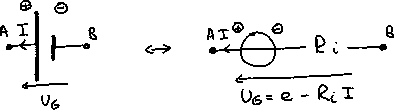
\includegraphics[width=0.5\textwidth]{figures/Corr05}
\end{center}

Ils savent que la puissance émis par la pile est donnée par :
\begin{align*}
P = e \cdot I - R \cdot I^2
\end{align*}
où $e$ est la f.e.m., $R$ est la résistance interne.

Afin de minimiser le terme associé à l'effet Joule/chute ohmique, les étudiants doivent proposer le couple rédox maximisant la f.e.m. : 
\begin{align*}
e &\approx e^\circ \approx  E^\circ_\oplus - E^\circ_\ominus \\
&\approx E^\circ ( \ce{Ag+ / Ag} ) - E^\circ ( \ce{Al^{3+} / Al} ) \\
&\stackrel{AN}{=} 2.42 ~ \si{\volt}
\end{align*}
Le couple \ce{Ag+ / Ag} et \ce{Al^{3+} / Al} présentent la meilleur qualité d'énergie en théorie.
\end{solution}
\end{framed}

L'aluminium est un métal qui a tendance à se passiver naturellement au contact de l'eau. La passivation est un Afin de comperndre ce qu'il peut se passer, on se propose d'étudier le diagramme de Poubaix de cet élément au contact d'un milieu aqueux : 

\begin{center}
\begin{minipage}{0.58\textwidth}

\includegraphics[width=\textwidth]{figures/Fig04}
\end{minipage}\begin{minipage}{0.38\textwidth}
\captionof{figure}{Diagramme E-pH de l'aluminium et de l'eau à \SI{25}{\celsius} [la convention de tracé est fixée à \SI{1}{\mole\per\liter}]}
\label{fig:04}
\end{minipage}
\end{center}

\begin{framed}
\question[\half] \label{Q:04} Définir le terme \og passivation naturelle \fg{}.  En vous appuyant sur la Fig. \ref{fig:04}, argumenter la nature chimique de la couche de passivation. Faites un schéma d'une plaque d'aluminium et représenter la couche de passivation. En quoi est-ce un soucis pour la réalisation d'une pile ?

\begin{solution}[2cm]
Protection d'un métal ou d'un alliage métallique contre la corrosion grâce à la formation d'une couche d'oxyde protectrice.\\

Dans le cas de l'aluminium, la passivation s'obtient naturellement au contact de l'eau ou de l'air.\\

Le diagramme de Poubaix nous renseigne sur les domaines de stabilité thermodynamique de l'aluminium, oxyde et hydroxyde au contact de l'eau (corrosion humide). \`{A} pH autour de 7, on observe que l'aluminium se corrode au contact de l'eau, sous forme d'hydroxydes d'aluminium ou d'oxydes d'aluminium, communément appelé alumine. 

Un schéma analogue au suivant peut être proposé : 
\begin{center}
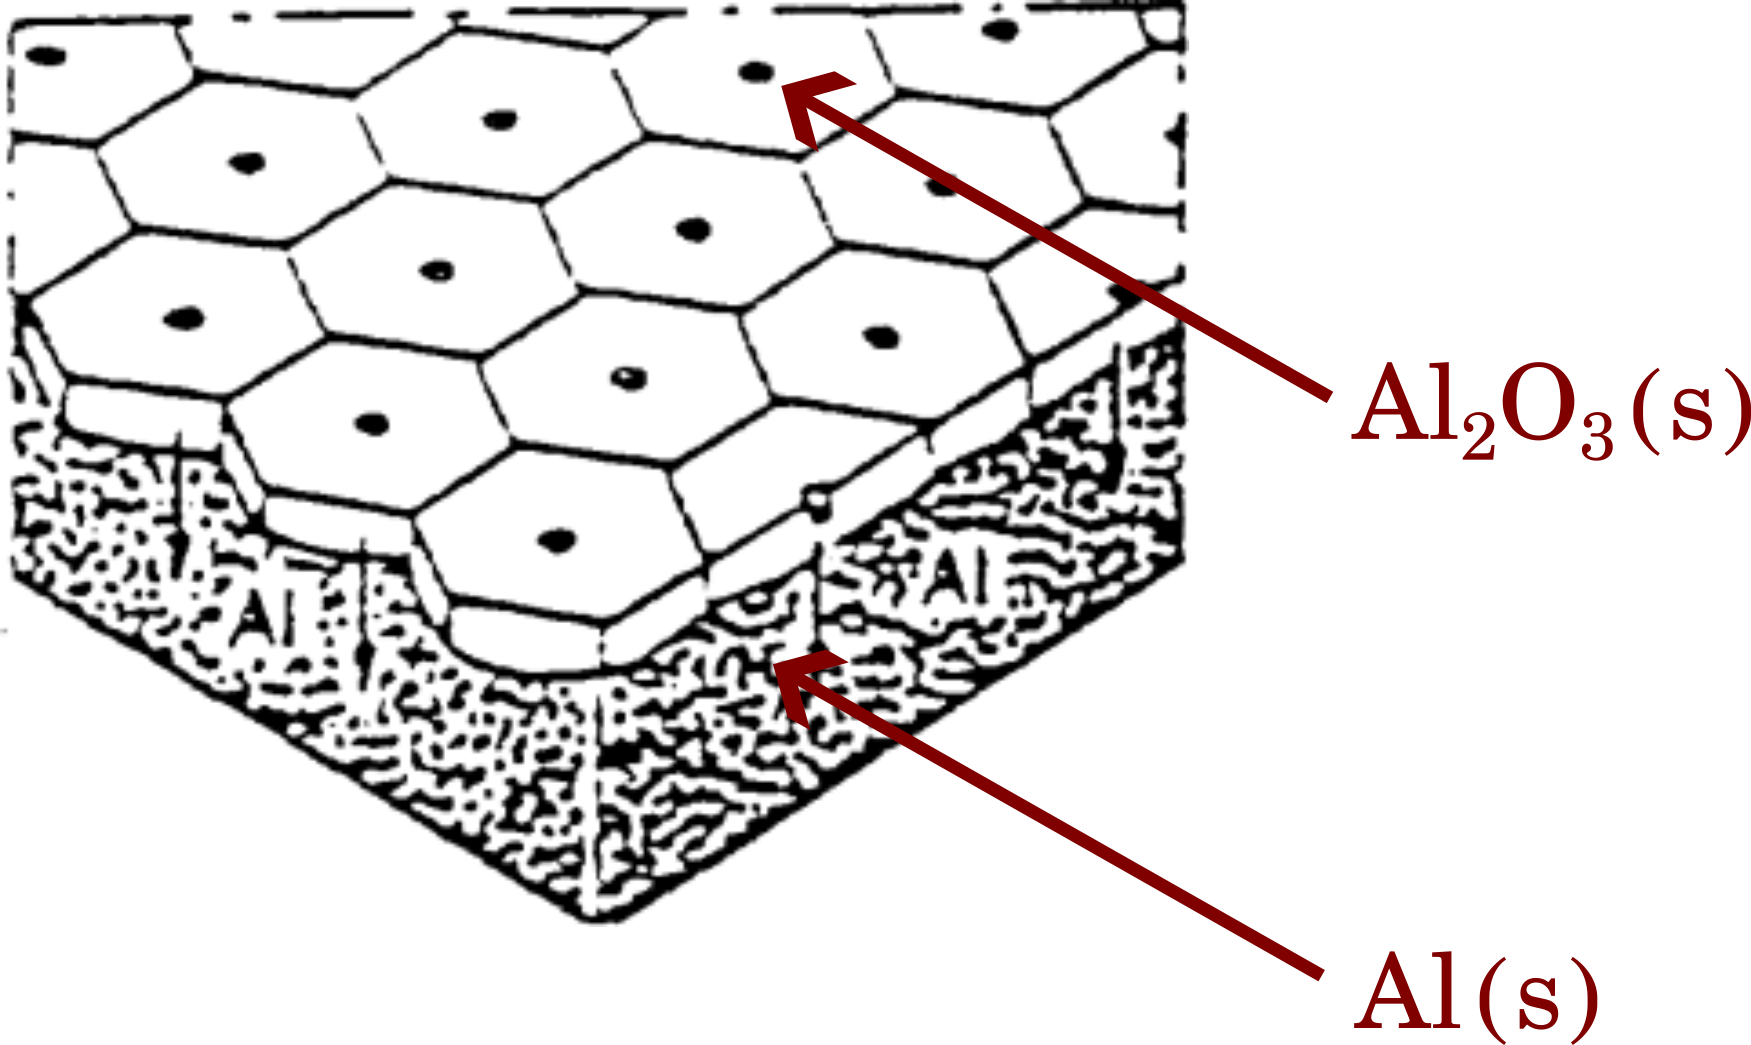
\includegraphics[height=3cm]{figures/Corr04}
\end{center}%Vigne, Une vie d'aluminium

L'apparition de l'alumine pose deux soucis technique pour réaliser :
\begin{enumerate}
\item l'aluminium n'est plus en contact avec les ions aluminium (isolant ionique) ;
\item l'aluminium ne permet pas le passage des électrons (isolant électronique) vers le circuit électrique.
\end{enumerate}

\end{solution}
\end{framed}

Du fait des contraintes matériel, dans la suite du sujet, nous nous limiterons à l'étude du couple \ce{Zn}/\ce{Cu}.

\setcounter{foo}{\value{question}}
\end{questions}

\paragraph*{Données} 
\begin{itemize}
\item Potentiel standard en \si{\volt\per{ESH}} à \SI{298}{\kelvin} :
\begin{center}
\begin{tabular}{cccccc}
\toprule
Couple & \ce{Ag+ / Ag} & \ce{Cu^{2+} / Cu} & \ce{Fe^{2+} / Fe} & \ce{Zn^{2+} / Zn} & \ce{Al^{3+} / Al} \\
\midrule
$E^\circ $ & 0.80 & 0.34 & -0.44 & -0.76 & -1.66 \\
\bottomrule
\end{tabular}
\end{center}

\item Résistivité électrique de quelques matériaux à \SI{293}{\kelvin} :
\begin{center}
\begin{tabular}{cccccc}
\toprule
Couple & Al & \ce{Al2O3} \\
\midrule
$\rho ~ [\si{\ohm\meter}] $ & $10^{-3}$ & $10^{12}$ \\
\bottomrule
\end{tabular}
\end{center}
\end{itemize}

Cette section comporte {\thefoo} questions pour un total de {\numpoints} points sur 20.

\newpage

\section{Détermination de grandeurs thermodynamique et cinétique de cellules électrochimiques - \faClockO ~ \SI{1}{\hour}\SI{30}{\minute}}

\subsection{Mesure de la force électromotrice}

\paragraph*{Schéma du montage}
\begin{center}
\begin{minipage}{0.48\textwidth}

\includegraphics[width=\textwidth]{figures/Fig01}
\end{minipage}\begin{minipage}{0.48\textwidth}
\captionof{figure}{Montage expérimental permettant la mesure de la force électromotrice.}
\label{fig:01}
\end{minipage}
\end{center}

\paragraph*{Protocole expérimental}
\begin{enumerate}
\item Prendre deux béchers thermostatés de \SI{400}{\milli\liter}, les recouvrir de papier aluminium à l'extérieur afin de limiter les déperditions thermiques ;
\item Connecter en circuit fermé ces deux béchers au bain thermostaté, puis allumer la circulation d'eau ;
\item Régler le bain à \SI{20}{\celsius} ;
\item Verser \SI{100}{\milli\liter} d'une solution de sulfate de zinc et une solution de sulfate de cuivre dans chacun des béchers ;
\item Ajouter quelques gouttes d'acide sulfurique concentré et vérifier le pH ;
\item Installer les électrodes, les connectiques, le pont salin de \ce{KNO3} et le thermomètre dans un des béchers ;
\item Installer le voltmètre.
\end{enumerate}

\subsection{Montage d'une pile Zn|Cu}
\begin{questions}
\setcounter{question}{\thefoo}
\begin{framed}
\question[\half] Représenter en notation simplifiée le montage chimique de la pile.

\begin{solution}[2cm]
On indique par $|$ les interfaces et par $\ominus/\oplus$ les pôles à l'aide de l'étude de corrosion de la partie précédente.

\begin{equation*}
\ominus ~ \ce{Zn (s)} | \ce{Zn^{2+} (aq)} ; \ce{SO_4^{2-} (aq)} | \ce{K^+ (aq)} ; \ce{NO_3^{2-} (aq)} | \ce{Cu^{2+} (aq)} ; \ce{SO_4^{2-} (aq)} | \ce{Cu (s)} ~ \oplus
\end{equation*}
\end{solution}
\end{framed}

\begin{framed}
\question[\half] \`{A} l'aide du voltmètre, vérifier la polarité de la pile et relever la tension à courant nul. Schématiser les deux situations puis compléter la question précédente.

\begin{solution}[2cm]

\begin{figure}[H]
\begin{center}
\subfloat[\label{fig:Corr02a}]{
\includegraphics[width=3cm]{figures/Corr02a}}\hspace{1cm}\subfloat[\label{fig:Corr02b}]{
\includegraphics[width=3cm]{figures/Corr02b}}
\caption{\ref{fig:Corr02a} Circuit équivalent permettant d'obtenir une tension positive ; \ref{fig:Corr02b} Circuit équivalent permettant d'obtenir une tension négative.}
\end{center}
\end{figure}

Les étudiants trouvent autour de \SI{1.1}{\volt}.


En changeant l'orientation du voltmètre, les étudiants remarquent que la tension indiquée est positive (voir Fig. \ref{fig:Corr02a}) ou négative (voir \ref{fig:Corr02b}), ils peuvent confirmer la polarité de la pile.
\end{solution}
\end{framed}

\begin{framed}
\question[\half] Complèter le schéma de la Fig.\ref{fig:01} en décharge en indiquant : la polarité, le sens du courant et de circulation des électrons ainsi que l'anode et la cathode. Donner les demi-équations rédox associé à chaque demi-pile.
\begin{solution}
\begin{center}

\includegraphics[width=8cm]{figures/Corr03}
\begin{minipage}{0.48\textwidth}
\begin{align*}
\ce{Zn (s, \ominus) = Zn^{2+} (aq, \ominus) + 2e^-}
\end{align*}
\end{minipage}\begin{minipage}{0.48\textwidth}
\begin{align*}
\ce{Cu^{2+} (aq, \oplus) + 2e^- = Cu(s, \oplus)}
\end{align*}
\end{minipage}\end{center}
\end{solution}

\end{framed}

\begin{framed}
\question[\half] En déduire l'équation de réaction fictive associée à cette pile.
\begin{solution}
\begin{center}
\begin{minipage}{0.4\textwidth}
\begin{align*}
\ce{Zn (s, \ominus) + Cu^{2+} (aq, \oplus) =  Zn^{2+} (aq, \ominus) + Cu(s, \oplus)}
\end{align*}
\end{minipage}
\end{center}

\end{solution}
\end{framed}
\setcounter{foo}{\value{question}}
\end{questions}

\subsection{Caractéristique et interprétation}

\subsubsection{Tracé de la caractéristique et confrontation au modèle linéaire}

\paragraph*{Schéma du montage}

\begin{center}
\begin{minipage}{0.48\textwidth}

\includegraphics[width=\textwidth]{figures/Fig07}
\end{minipage}\begin{minipage}{0.48\textwidth}
\captionof{figure}{Montage de base de l'expérience.}
\label{fig:07}
\end{minipage}
\end{center}

\paragraph*{Matériel à votre disposition}

En plus du matériel indiqué à la Fig. \ref{fig:07}, on met à votre disposition le matériel suivant : 
\begin{itemize}
\item quatre multimètres ;
\item des fils ; 
\item deux électrodes au calomel saturée ;
\end{itemize}



\begin{questions}
\setcounter{question}{\thefoo}
\begin{framed}
\question[1] Placer dans le dispositif expérimental de la Fig. \ref{fig:07}, les électrodes de référence et les voltmètre pour mesurer : le potentiel d'électrode $\oplus$, le potentiel d'électrode $\ominus$ et l'ensemble (potentiel de jonction + tension de résistance dans la pile). Ajouter ensuite le dernier ampèremètre afin de faire l'acquisition du courant, de telle sorte que la \textbf{pile Daniell soit en convention générateur}. Un ou des schémas expérimentaux sont attendus.
\begin{solution}

\begin{center}
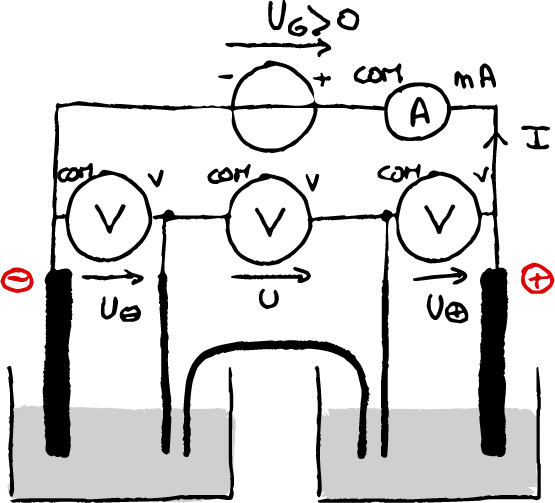
\includegraphics[width=0.48\textwidth]{figures/Corr06a}\hfill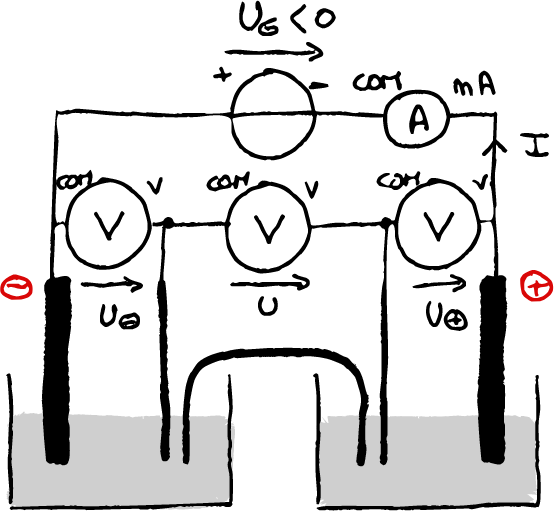
\includegraphics[width=0.48\textwidth]{figures/Corr06b}
\captionof{figure}{Le montage à gauche permet la mesure des tensions positives de la pile, le montage de droite des tensions négatives de la pile}
\end{center}

\end{solution}
\end{framed}

\question[1] Appeler l'enseignement pour qu'il vérifie le montage électrique et chimique.

\begin{framed}
\question[1] Décomposer le potentiel électrostatique entre la borne $\oplus$ et $\ominus$ de la pile, et démontrer que l'on fait bien l'acquisition des potentiels demandés.
\begin{solution}
On peut décomposer le potentiel électrostatique : 
\begin{align*}
U_G &= \Phi_\oplus - \Phi_\ominus \\
&= \underbrace{(\Phi_\oplus - \Phi_{S_\oplus})}_{E_\oplus} + \underbrace{(\Phi_{S_\oplus} - \Phi_{ECS_\oplus})}_{-E_{ECS,\oplus}} + \underbrace{(\Phi_{ECS_\oplus} - \Phi_{ECS_\ominus})}_{U} - \underbrace{(\Phi_{S_\ominus} - \Phi_{ECS_\ominus})}_{-E_{ECS,\ominus}} - \underbrace{(\Phi_{\ominus} - \Phi_{S_\ominus})}_{E_\ominus} \\
&= (E_\oplus [\si{\volt\per{ESH}}] - E_{ECS, \oplus} [\si{\volt\per{ESH}}]) + U - (E_\ominus [\si{\volt\per{ESH}}] - E_{ECS, \ominus} [\si{\volt\per{ESH}}]) \\
U_G &= E_\oplus [\si{\volt\per{ECS}}] + U - E_\ominus [\si{\volt\per{ECS}}]
\end{align*}
Lors de la mesure, on a trois tensions : 
\begin{itemize}
\item la tension $U_\oplus$ assimilable au potentiel à la $E_\oplus$ par rapport à l'ECS ;
\item la tension $U$ assimilable à la chute ohmique ;
\item la tension $U_\ominus$ assimilable à l'inverse du potentiel $E_\ominus$ par rapport à l'ECS.
\end{itemize}

\end{solution}
\end{framed}

Dans le cas d'un générateur de tension Owon ODP3031, régler le courant Curr/CC à \SI{3.0}{\ampere}. L'Owon est assimilable à un générateur de tension. Faites varier la tension au générateur entre \SI{-8}{\volt} et \SI{8}{\volt} par pas de \SI{0.5}{\volt}, réaliser la mesure du courant électrique et des trois tensions de la partie précédente. 

\faWarning ~ La tension aux bornes du cuivre fluctue beaucoup et il est difficile de la stabiliser. \`{A} un moment, il faut se lancer et faire la mesure à un instant $t$, il est inutile d'attendre une stabilisation qui n'arrivera pas.

\begin{framed}
\question[1\half] Représenter l'évolution de la caractéristique $(I, U_G)$ expérimentale. Vous penserez à ajouter une légende, des axes et un titre à votre graphe.
\begin{solution}
Les étudiants vont le courant $I$ mesuré à l'ampèremètre en fonction de la grandeur :
\begin{align}
U_G = U_\oplus + U + U_\ominus 
\end{align}
Il obtiennent le graphe suivant : 

\begin{center}
\begin{minipage}{0.48\textwidth}

\includegraphics[width=\textwidth]{figures/Graph01}
\end{minipage}\begin{minipage}{0.48\textwidth}
\captionof{figure}{Caractéristique expérimentale associée à}
\end{minipage}
\end{center}
\end{solution}
\end{framed}

On rappelle qu'une modélisation commune du fonctionnement d'une pile consiste à modéliser la pile à un \textbf{dipôle linéaire} résultant de l'association d'un générateur de tension de force électromotrice $e$ et d'une résistance de tension $U$.

\begin{center}

\includegraphics[width=0.9\textwidth]{figures/Fig06}
\captionof{figure}{Modélisation de la pile à un dipôle linéaire résultant de l'association d'un générateur de tensionet d'une résistance interne.}
\label{fig:06}
\end{center}

La force électromotrice est la tension prédite par la thermodynamique, tandis que la résistance interne prend en compte les phénomènes dissipatifs associés à la circulation des ions (dans les solutions et le pont salin) ou des électrons (dans les plaques). 

\begin{framed}
\question[1\half] Reproduire la fig. \ref{fig:06} et orienter les tensions élctriques. Exprimer $U_G$ la tension aux bornes de la pile en fonction de la force électromotrice $U_G (I=0 ~ \si{\ampere})$, de la résistance $R$ et du courant $I$. En vous appuyant sur une des tensions mesurées précédemment, déterminer la résistance interne de la pile.
\begin{solution}

Le modèle de Thévenin nous permet d'écrire la caractéristique de la pile comme : 
\begin{align*}
U_G (I) &= U_G(I=0) + U \\
&= U_G(I=0) - R \cdot I
\end{align*}

Dans notre expérience, on a estimé le terme résistif. Ce terme est associé à $U$ d'équation : 
\begin{align*}
U &= \Phi_{ECS_\oplus} - \Phi_{ECS_\ominus} \\ 
&= - R \cdot I
\end{align*}

On peut donc tracer la caractéristique associée à la résistance interne et la modélisée à l'aide d'une équation linéaire :
\begin{center}
\begin{minipage}{0.48\textwidth}
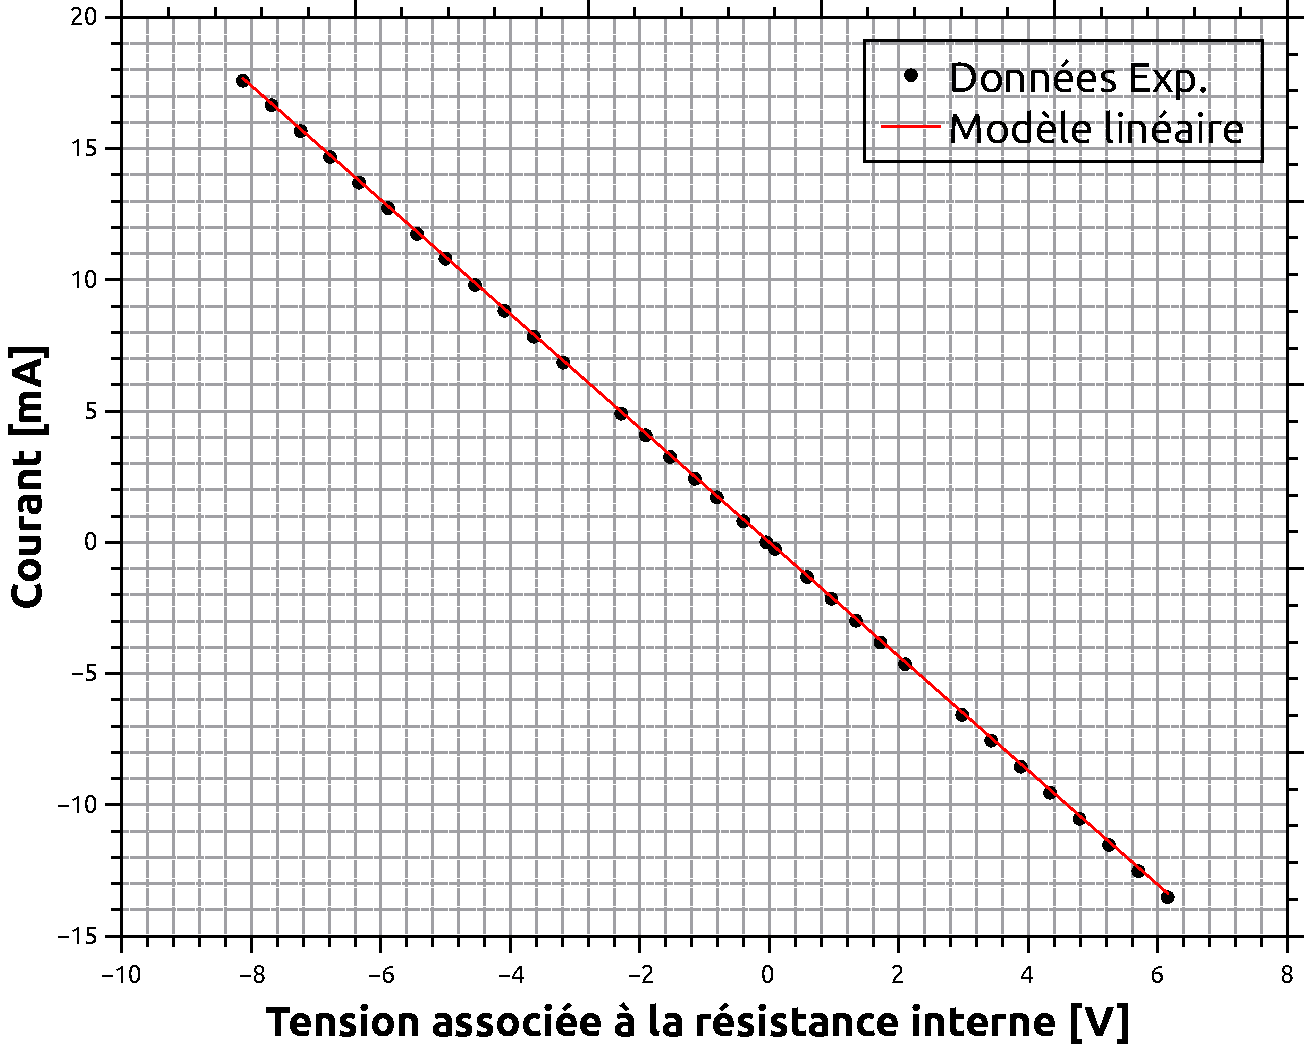
\includegraphics[width=\textwidth]{figures/Graph04}
\end{minipage}\hspace{0.2cm}\begin{minipage}{0.48\textwidth}
\captionof{figure}{Caractéristiques de la résistance interne associée à la pile Daniell maintenue à \SI{24.9}{\celsius}. Un modèle linéaire passant par (0,0) a été utilisé pour trouver la conductance.}
[Matériel : Acquisition avec un multimètre Meteix MX 554, deux électrodes de référence ECS dans les conditions de l'énoncé, analyse : Qtiplot]
\end{minipage}
\end{center}

Le modèle linéaire est partiellement validé : points alignés, $R^2 = 0.999049021\ldots$. Cependant, on remarque qu'il y a un léger biais dans la mesure du potentiel.

\begin{align*}
I [\si{\milli\ampere}] = (-2.17 \cdot 0.02) U [\si{\volt}]
\end{align*}

On trouve alors que la résistance vaut : 
\begin{align*}
R = (461 \pm 5) ~ \si{\ohm}
\end{align*}

\textbf{Nota Bene :} Les étudiants ne penseront pas à prendre en compte le biais statistique largement observé qui est dû à deux choses : 
\begin{enumerate}
\item une légère tension (biais de tension, noté $U_{biais}$) existant entre les deux ECS, laquelle a été évaluée autour de $25.4 \si{\milli\volt}$ ;
\item l'existence d'un potentiel de jonction $E_j$ à courant nul.
\end{enumerate}
Une modélisation de la forme : 
\begin{align*}
U - U_{biais} = E_j - R \cdot I
\end{align*}
Vous pouvez potentiellement discuter de ces paramètres avec les étudiants qui n'ont pas de difficultés. Cependant, ça ne doit pas être le c{\oe}ur de la discussion et ça ne doit pas leur faire perdre du temps.
\end{solution}
\end{framed}

\begin{framed}
\question[1] Superposer la caractéristique expérimentale à celle du modèle de Thévenin. En vous appuyant sur un résonnement énergétique, commenter le résultat obtenu.
\begin{solution}
Les étudiants doivent superposer le modèle de Thévenin aux points expérimentaux :
\begin{center}
\begin{minipage}{0.48\textwidth}

\includegraphics[width=\textwidth]{figures/Graph01}
\end{minipage}\begin{minipage}{0.48\textwidth}
\captionof{figure}{Caractéristique expérimentale et d'un modèle linéaire à \SI{24.9}{\celsius}.}
\end{minipage}
\end{center}

\textbf{Interprétation du graphe :}
\begin{center}
\begin{minipage}{0.48\textwidth}
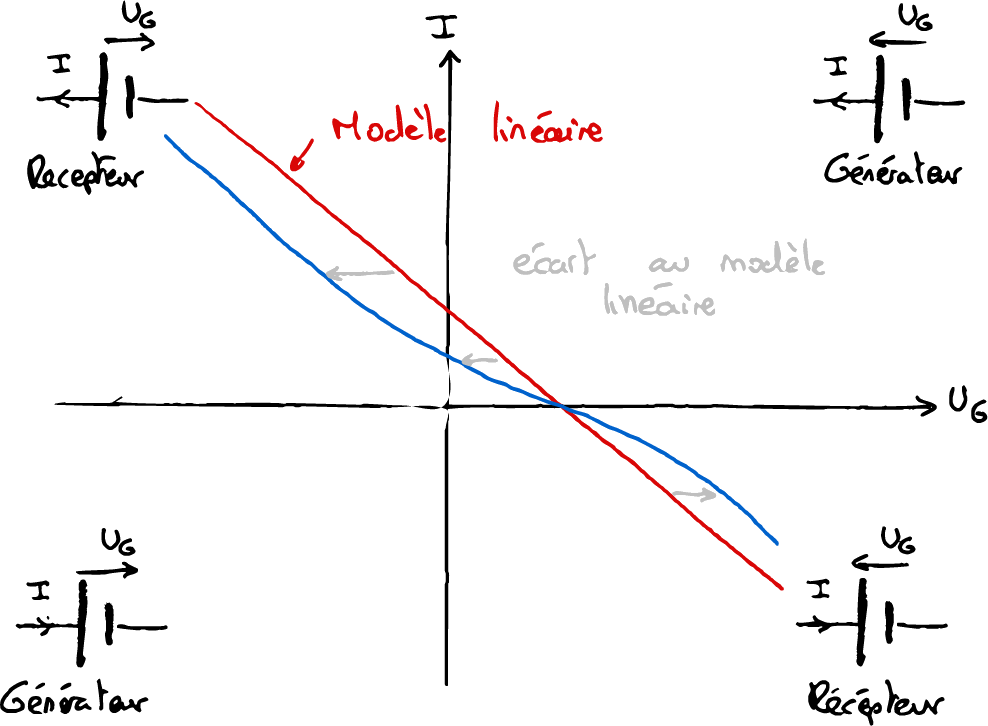
\includegraphics[width=\textwidth]{figures/Corr07}
\end{minipage}\begin{minipage}{0.48\textwidth}
\captionof{figure}{Interprétation de l'écart à linéarité.}
\end{minipage}
\end{center}


Plusieurs conclusions doivent être tirées : 
\begin{enumerate}
\item la caractéristique n'est pas du tout linéaire ;
\item la caractéristique se comporte comme suit : 
Lorsque la pile se comporte comme un générateur, à un courant donné, la tension du générateur est plus petite que la tension du modèle linéaire. Une partie de l'énergie du générateur est perdue. Lorsque la pile se comporte comme un récepteur, à un courant donné, la tension aux bornes du générateur est plus grande que la tension du modèle linéaire. Cela signifie qu'il faut fournir à la pile plus d'énergie que prédit.
\end{enumerate}
\textbf{Nota Bene :} Ne pas hésiter à aider les étudiants à bien comprendre le sens de chaque quadrant de la caractéristique. Il auront des difficultés à donner un sens "énergétique" aux tensions.
\end{solution}
\end{framed}
\setcounter{foo}{\value{question}}
\end{questions}

Par la suite, on va chercher à comprendre l'origine chimique du terme non linéaire en utilisant les potentiels rédox du cuivre et du zinc.

\subsubsection{\'{E}cart à la linéarité : courbe courant-potentiel}

Afin de prendre en compte l'écart à la linéarité, on va définir une nouvelle grandeur appelée surtension, qui prend en compte la différence entre le potentiel interfacial de l'électrode à courant non nul par rapport au courant nul : 
\begin{align*}
E_\oplus (I) &= E_{\oplus, eq} + \eta_a (I) \quad \text{avec }\eta_a (I) > 0 \\
E_\ominus (I) &= E_{\ominus, eq} + \eta_c (I) \quad \text{avec }\eta_c (I) < 0
\end{align*}
où l'indice $eq$ indique le potentiel d'équilibre, assimilable au potentiel de Nernst du couple mis en jeux dans la demi-pile.

\begin{questions}
\setcounter{question}{\thefoo}
\begin{framed}
\question[1] Représenter la courbe courant-potentiel attendu pour le cuivre et le zinc si le potentiel à chaque électrode était assimilé au potentiel thermodynamique. Vous utiliserez les conventions suivantes : 
\begin{align*}
I > 0 \implies \text{oxydation} ;\\
I < 0 \implies \text{réduction}.
\end{align*}
et vous prendre un potentiel rédox exprimé en $\si{\volt\per{ECS}}$.



\begin{solution}
Dans l'hypothèse thermodynamique, $\forall I, \quad \eta_a (I) = \eta_c (I) = 0$
\begin{align*}
E_\oplus (I) &=  E_{\oplus, eq} = E^\circ (\ce{Cu^{2+} (aq) / Cu(s)}) + \frac{\alpha}{2} \log \frac{[\ce{Cu^{2+}}]}{c^\circ} - E_{ECS} \\
E_\ominus (I) &=  E_{\ominus, eq} = E^\circ (\ce{Zn^{2+} (aq) / Zn(s)}) + \frac{\alpha}{2} \log \frac{[\ce{Zn^{2+}}]}{c^\circ} - E_{ECS}
\end{align*}
\textbf{Application Numérique :}
\begin{align*}
E_\oplus (I) &= 0.06 ~ \si{\volt\per{ECS}} \\
E_\ominus (I) &= -1.04 ~ \si{\volt\per{ECS}}
\end{align*}

On peut donc représenter la courbe courant-potentiel suivante dans un modèle \SI{100}{\percent} thermodynamique : 

\begin{center}
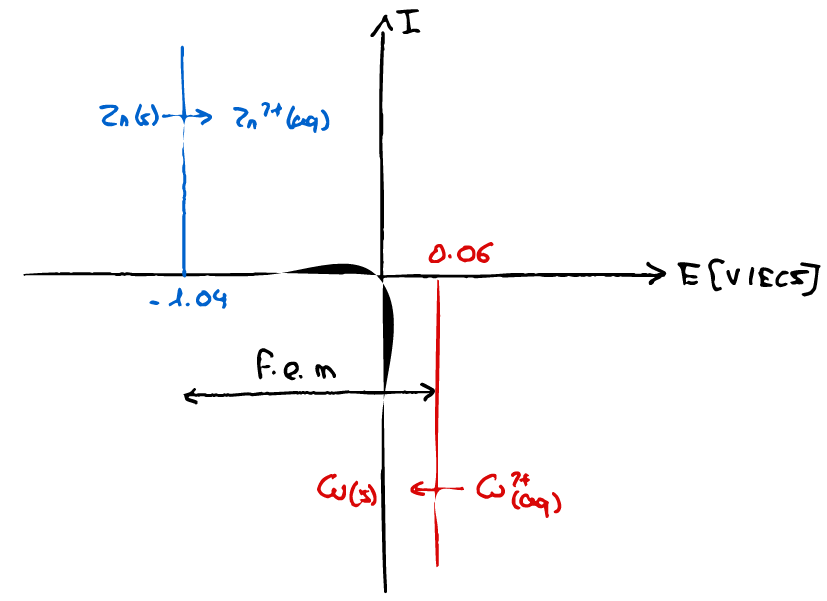
\includegraphics[width=0.48\textwidth]{figures/Corr08}
\end{center}

\end{solution}
\end{framed}

\begin{framed}
\question[1] Au modèle thermodynamique, vous superposerez le potentiel de chaque électrode en veillant à toujours respecter la convention suivante : 
\begin{align*}
I > 0 \implies \text{oxydation} ;\\
I < 0 \implies \text{réduction}.
\end{align*}
Représenter schématiquement les surtensions anodique $\eta_a$ et cathodique $\eta_c$ lorsque la pile fonctionne comme générateur. Quel peut-être l'origine chimique de ces surtensions ?

\begin{solution}

Les étudiants doivent veiller à orienter leurs tensions correctement. Avec le setting expérimental utilisé, on trouve bien : 
\begin{align*}
U_G &= E_{\oplus, eq} - E_{\ominus, eq} + \eta_c - \eta_a  - R \cdot I\\
&= 
\end{align*}

\begin{center}
\begin{minipage}{0.48\textwidth}
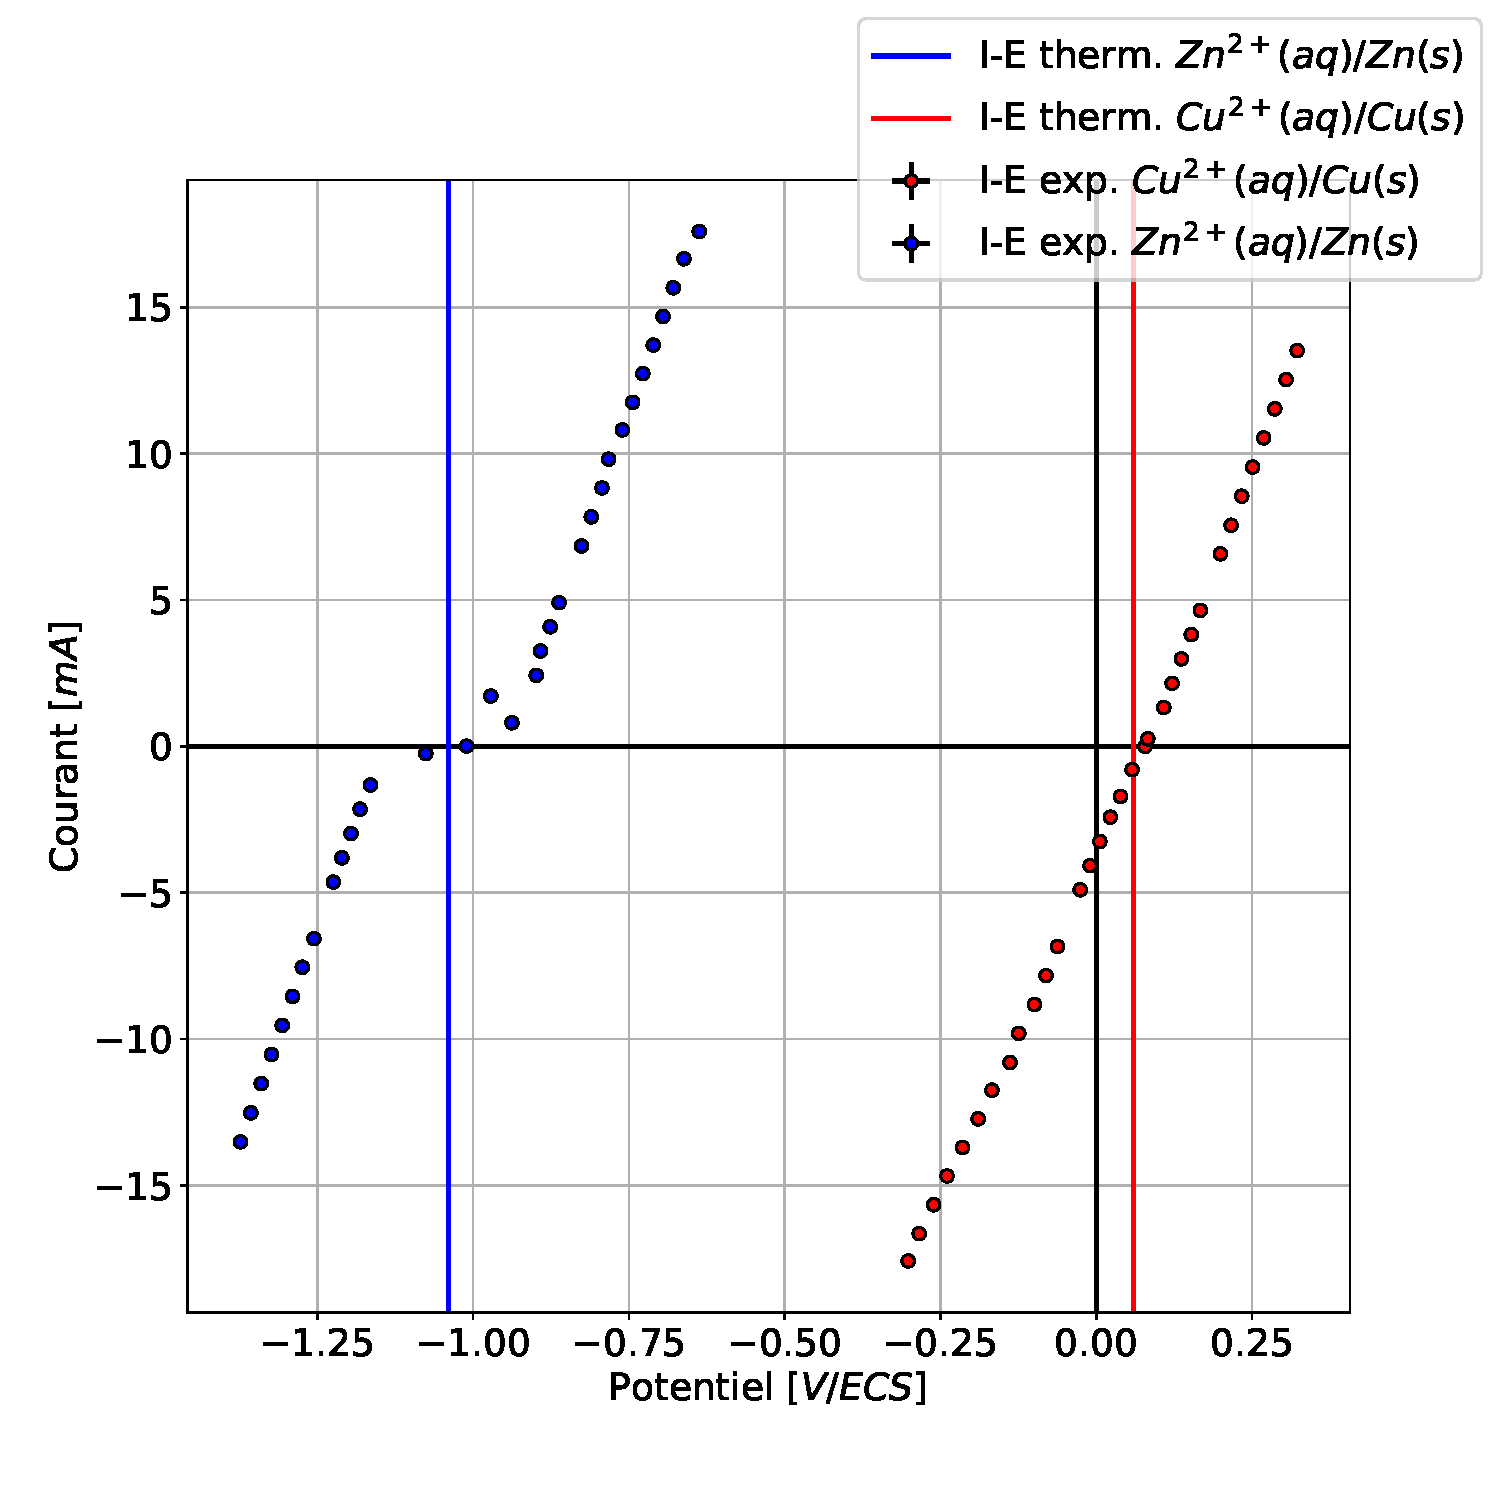
\includegraphics[width=\textwidth]{figures/Graph02}
\end{minipage}\begin{minipage}{0.48\textwidth}
\captionof{figure}{Courbe courant-potentiel à une électrode de cuivre et un électrode de zinc. Les points $\bullet$ représentent les données expérimentales, tandis que les lignes verticales représentent ce qui est prédit par la thermodynamique}
\end{minipage}
\end{center}
En ajoutant les surtensions au modèle de Thévenin, on a finalement pris en compte l'écart entre le potentiel thermodynamique et le potentiel oxydo-réduction : 
\begin{center}
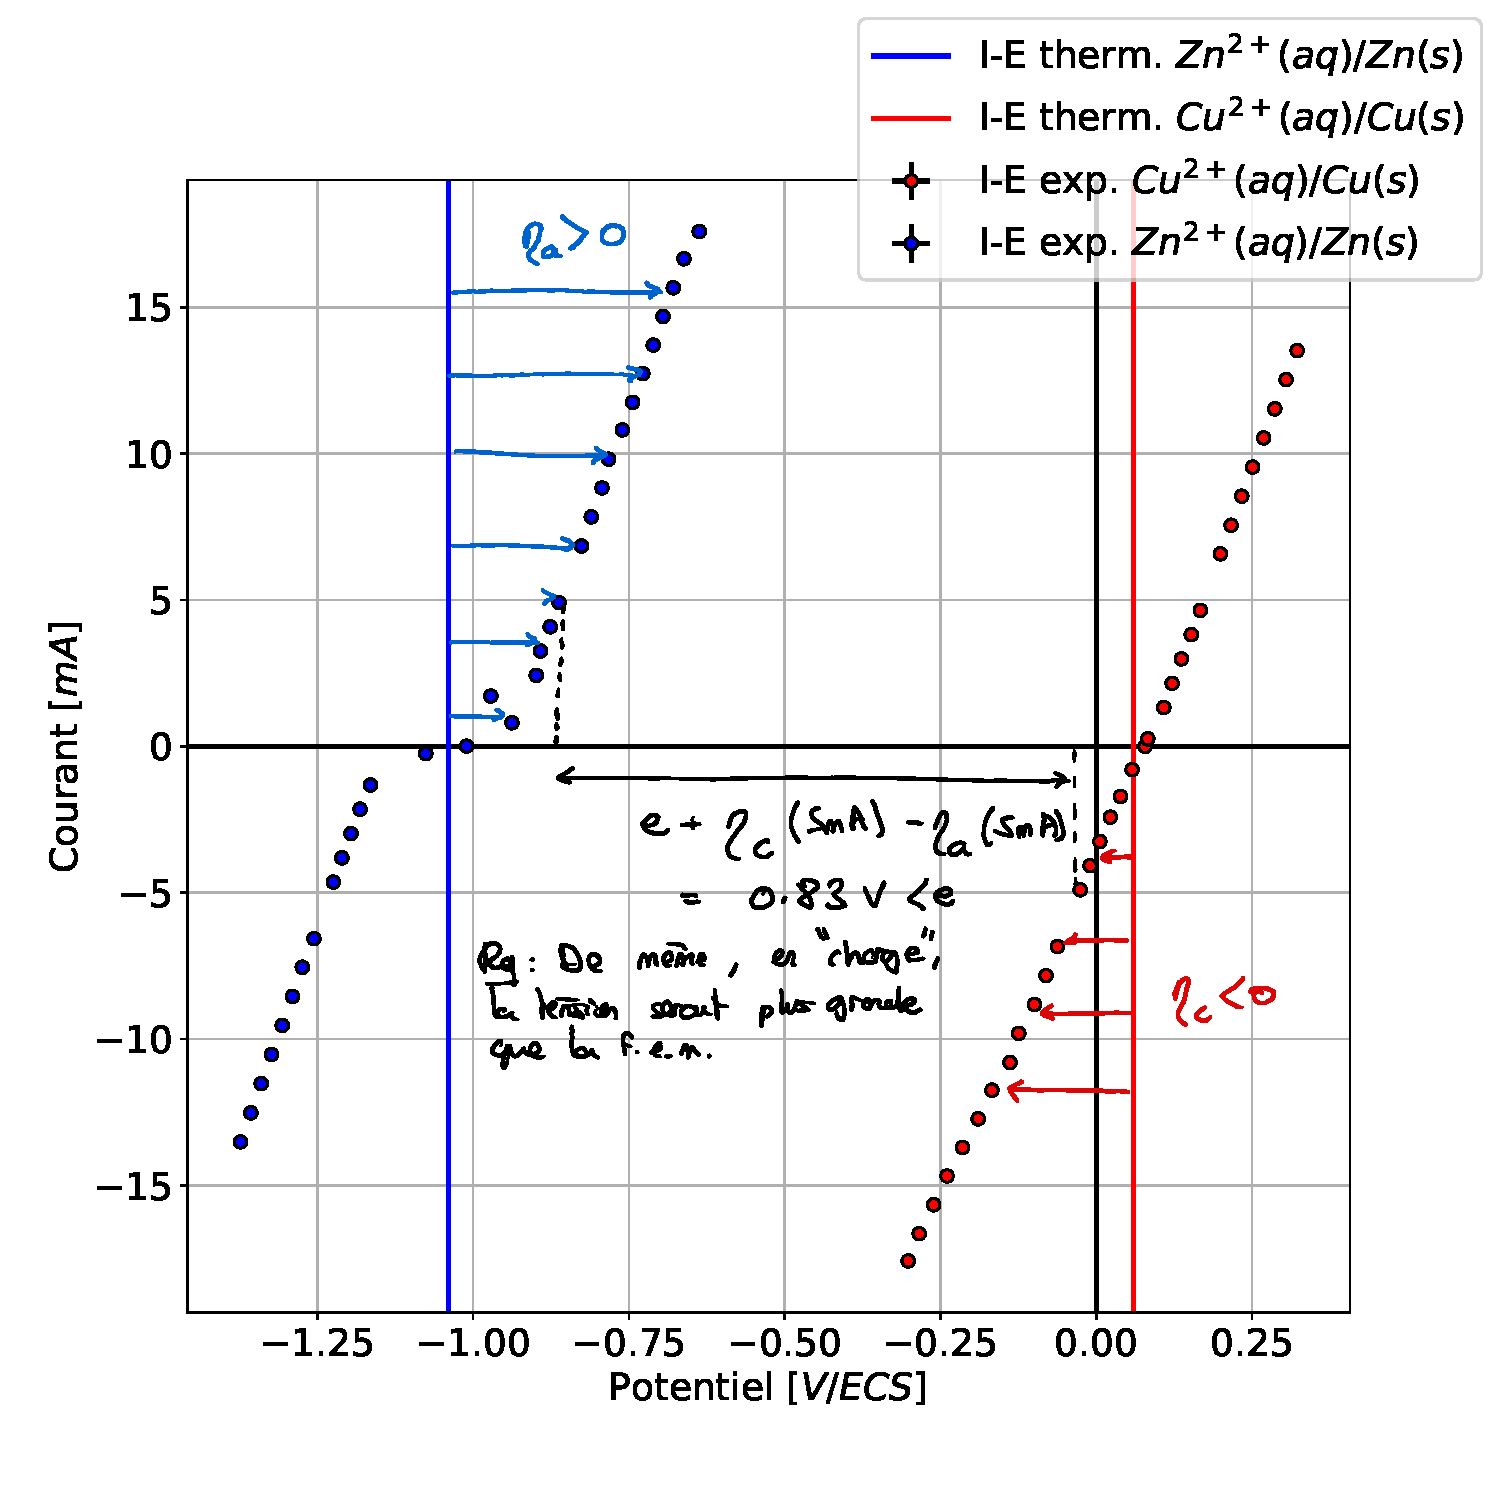
\includegraphics[width=0.48\textwidth]{figures/Graph02-bis}
\end{center}

Dans le cas du fonctionnement de la pile comme générateur, par exemple à I = \SI{5}{\milli\ampere}, la différence de potentiel entre les deux électrodes est plus faible que prédit et vaut \SI{0.83}{\volt}. Cela traduit le fait qu'une partie de l'énergie chimique libérée sert à franchir la barrière d'activation associée à l'oxydation (resp. la réduction) à la surface du zinc (resp. l'oxydation).

L'écart à la linéarité est d'origine \textbf{cinétique}.
\end{solution}
\end{framed}
\setcounter{foo}{\value{question}}
\end{questions}

\begin{comment}
Les étudiants doivent proposer un modèle type Thevenin composé d'un générateur de tension parfait et d'une résistance interne.

De ce modèle, les étudiants propose l'équation modèle suivante : 

\begin{equation*}
U_G (I)= e - R_i I \implies I (U_G) = \frac{e}{R_i} - \frac{1}{R_i} U_G
\end{equation*}
avec $e$ la tension à courant nul et $R_i$ la résistance interne.

Les étudiants pratiquent une régression linéaire et montrent que : 
\begin{itemize}
\item les points sont bien alignés ;
\item les points sont bien distribués autour de la droite ; 
\item le c{\oe}fficient de corrélation linéaire est proche de 1.
\end{itemize}
Ils concluent et valide leur modèle.

Un bonus pourra être donné à l'étudiant qui comparera la f.e.m. obtenue par le modèle à celle obtenue par une mesure directe.
\end{comment}

\subsection{Détermination des grandeurs thermodynamiques associées à la réaction de la pile}

On cherche à déterminer les grandeurs thermodynamiques de réaction dans la pile Zn|Cu. Pour cela, on rappelle que le comportement en température de la force électromotrice de la réaction est donnée par :

\begin{equation}
e (T) = \frac{\Delta_r S}{nF} T - \frac{\Delta_r H}{nF} 
\label{eq:e_T}
\end{equation}
avec $n$ le nombre d'électron échangé et $F$ la constante de Faraday.

Débrancher le dispositif électrique précédent et rebrancher le voltmètre, correctement orienté, aux bornes de la pile. Faites varier la température du bain de 20 à \SI{60}{\celsius}, par pas de \SI{5}{\celsius} et mesurer la tension à courant nul à chaque pas de température.

\faWarning ~ Il est inutile de perdre du temps à atteindre une équilibration à la température cible du bain. Vous pouvez annoter la température et la f.e.m. à l'aide d'un thermomètre plongé dans un compartiment de la pile.



\begin{questions}
\setcounter{question}{\thefoo}

\question[\half] Appeler l'enseignement pour qu'il vérifie le montage électrique et chimique.

\begin{framed}
\question[\half] \`{A} quelle condition, l'Eq. \ref{eq:e_T} donne-t-elle une droite ? 


\begin{solution}
Si on étudie la variation de la f.e.m. sur une plage étroite de température, il se peut que le couple $(\Delta_r H, \Delta_r S)$ varie peu. Dans ce cas, on peut appliquer l'approximation d'Ellingham et considérer ces deux paramètres comme constants.
\end{solution}

\end{framed}

\begin{framed}
\question[\half] En vous appuyant sur les relations démontrées à l'annexe \ref{sec:DrH&DrS}, justifier que dans la pile Daniell les grandeurs de réaction sont assimilables aux grandeurs de réaction standard : 


\begin{solution}
Dans le cas de l'idéalité, on a $Q = \frac{[\ce{Zn^{2+}}]}{[\ce{Cu^{2+}}]}$. Puisque les deux compartiments sont théoriquement à la même concentration, et en utilisant la relation \ref{eq:DrS-DrS°}, on trouve immédiatement que :
\begin{align*}
\Delta_r S \approx \Delta_r S^\circ
\end{align*}
Avec la relation \ref{eq:DrH-DrH°}, on a aussi : 
\begin{align*}
\Delta_r H \approx \Delta_r H^\circ
\end{align*}
Par conséquent, la force électromotrice est assimilable à la force électromotrice en condition standard, et l'Eq. \ref{eq:e_T} peut se réecrire comme : 
\begin{equation}
e (T) = e^\circ (T) \approx \frac{\Delta_r S^\circ}{nF} T - \frac{\Delta_r H^\circ}{nF} 
\end{equation}

\end{solution}

\end{framed}

\begin{framed}
\question[1\half] Tracer l'évolution de la f.e.m. de la pile. Appliquer cette condition et en déduire les paramètres thermodynamiques de réaction.


\begin{solution}
La courbe obtenue est la suivante : 
\begin{center}
\begin{minipage}{0.48\textwidth}
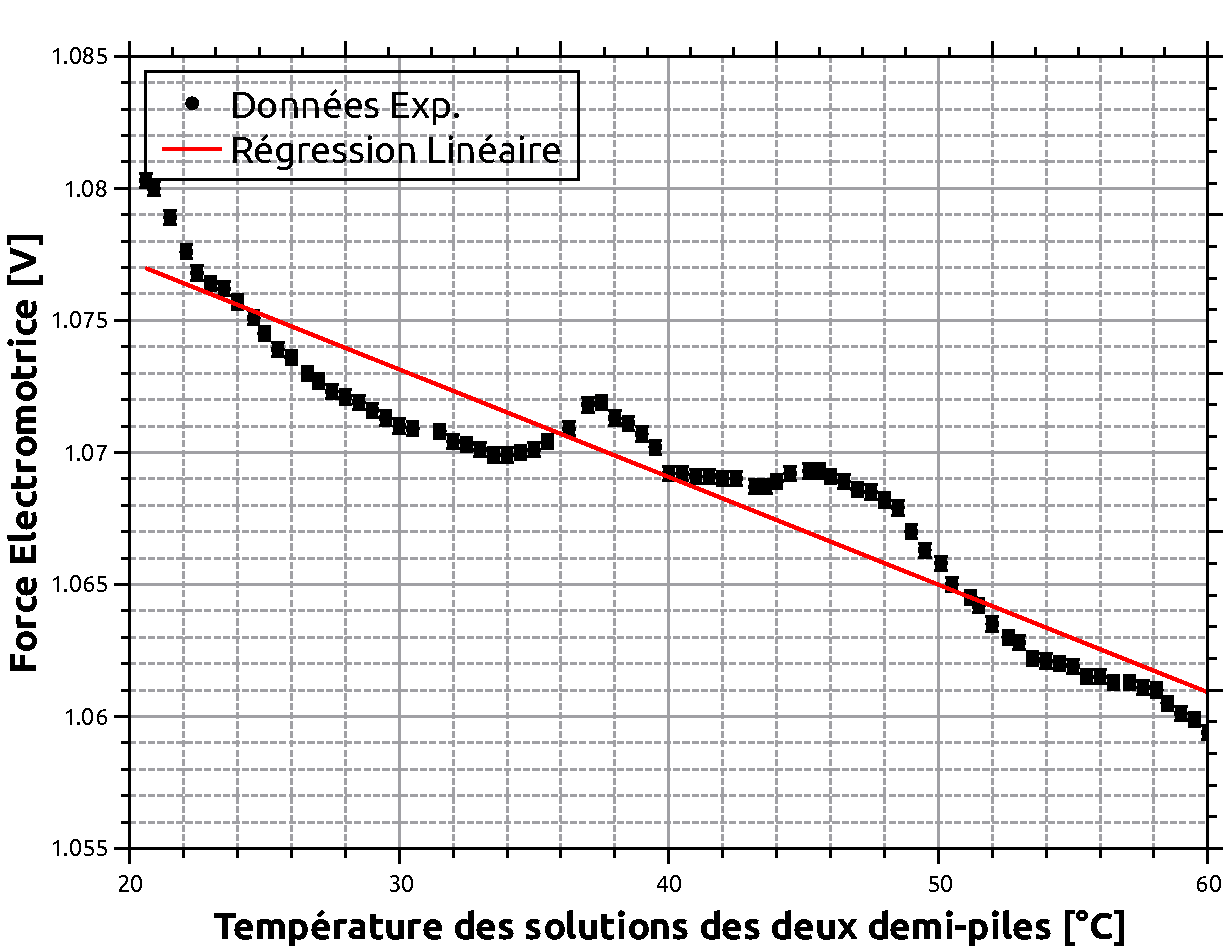
\includegraphics[width=\textwidth]{figures/Graph03}
\end{minipage}\hspace{0.2cm}\begin{minipage}{0.48\textwidth}
\captionof{figure}{\'{E}volution de la force électromotrice en fonction de la température dans un dispositif thermostaté.}
[Acquisition : multimètre Fluke 45, thermomètre Hanna HI 145 ; pile : cf. conditions opératoires, Traitement des données : Qtiplot]
\end{minipage}
\end{center}
Les étudiants tracent l'équation : 

\begin{equation*}
e^\circ (T) = \text{pente} \cdot T + \text{origine} 
\end{equation*}

avec $\text{pente} = \frac{\Delta_r S^\circ}{2F}$ et $\text{origine} = -\frac{\Delta_r H^\circ}{2F}$.

Avec les données ci-dessus, la courbe a pour équation : 
\begin{align}
e^\circ (T) (-4.1 \pm 0.2) \cdot 10^{-5} T + (1.196 \pm 0.005)
\end{align}

Encore une fois, ils valident leur modèle :
\begin{itemize}
\item en regardant la dispersion des résidus autour de la droite modèle ;
\item en regardant la distance des points à la droite modèle
\item en interprétant le $R^2$ au minimum.
\end{itemize}

Ici, on a des fluctuations surprenantes en température. Il doit y avoir un léger biais dû au contact du thermomètre avec l'électrode de zinc lors de l'acquisition. Ce biais ne devrait pas être présent avec les pièces d'acquisitions.

Cependant, le $R^2$ n'est pas trop mauvais ($\sim 0.09705$) et le $\chi^2 / dof \approx 4 \cdot 10^{-5}$ (chi2 réduit par le nombre de degré de liberté) est petit devant $1$, ce qui suggère un bon modèle de régression, mais avec des incertitudes sur-estimées. 

\begin{align*}
\Delta_r S^\circ &= (-7.9 \pm 0.4) \si{\joule\per\kelvin\per\mole} \\
\Delta_r H^\circ &= (-231 \pm 1) \si{\kilo\joule\per\mole} \\
\end{align*}
\end{solution}
\end{framed}

\begin{framed}
\question[1] En vous appuyant sur les données fournies, comparer la valeur obtenue à ce que prédise les grandeurs thermodynamiques tabulées. Interpréter les éventuels écarts observés.


\begin{solution}
Les étudiants partent de l'équation de réaction fictive : 
\begin{align*}
\ce{Zn (s) +  Cu^{2+} (aq) = Zn^{2+} (aq) + Cu (s)}
\end{align*}

et utilisent la loi de Hess : 

\begin{align*}
\Delta_r H^\circ &= \Delta_f H^\circ ( \ce{Zn^{2+} (aq)} ) - \Delta_f H^\circ ( \ce{Cu^{2+} (aq)} ) \\
\Delta_r S^\circ &= S^\circ ( \ce{Cu (s)} ) + S^\circ ( \ce{Zn^{2+} (aq)} ) - S^\circ ( \ce{Cu^{2+} (aq)} ) - S^\circ ( \ce{Zn (s)} ) 
\end{align*}

pour en déduire qu'à \SI{298}{\kelvin}, 
\begin{align*}
\Delta_r H^\circ = - 219 ~ \si{\kilo\joule\per\mole} \quad \Delta_r S^\circ = -19.9 ~ \si{\joule\per\mole\per\kelvin}
\end{align*}

On peut calculer l'écart relatif :
\begin{align}
\frac{\Delta_r H^\circ_{exp} - \Delta_r H^\circ_{theo}}{\Delta_r H^\circ_{theo}} &\approx 6 ~ \si{\percent} \\
\frac{\Delta_r S^\circ_{exp} - \Delta_r S^\circ_{theo}}{\Delta_r S^\circ_{theo}} &\approx 61 ~ \si{\percent} \\
\end{align}

On constate en somme que l'écart relatif sur l'entropie est assez grand. Ceci peut probablemet être mis en relation avec la vitesse d'acquisition de la f.e.m., laquelle n'a pas réellement été acquise en laissant le système s'équilibrer à chaque température. Avec un temps d'expérience plus grand, on pourrait éventuellement affiner la mesure.

L'écart en enthalpie est probablement dû au fait que le courant traversant la pile n'est pas tout à fait $0$, le voltmètre n'étant pas idéal. Cependant, le biais ne doit pas venir uniquement de là puisque l'on aurait sinon obtenu une f.e.m. plus petite, et donc une enthalpie plus grande que la valeur théorique. L'absence d'équilibration décrite précédemment doit aussi jouer un rôle, et compenser partiellement le biais systématique (ce qui explique la moindre erreur que l'entropie).
\end{solution}
\end{framed}
\setcounter{foo}{\value{question}}
\end{questions}

\paragraph*{Données}
\begin{itemize}
\item constante de Faraday : $F = 96485 ~ \si{\coulomb\per\mole}$
\item valeur d'un produit de constante à \SI{298}{\kelvin} : $\alpha = RT/F \ln 10 = \SI{59}{\milli\volt}$
\item Potentiel d'une électrode au calomel saturé à \SI{298}{\kelvin} : $E_{ECS} \approx \SI{0.25}{\volt\per{ESH}}$
\item Enthalpie de formation et d'entropie molaire à \SI{298}{\kelvin} des différentes espèces impliquées dans la réaction :
\begin{center}
\begin{tabular}{cccccc}
\toprule
Espèce & & \ce{Cu(s)} & \ce{Zn(s)} & \ce{Cu^{2+} (aq)} & \ce{Zn^{2+} (aq)} \\
\midrule
$\Delta_f H^\circ$ & [\si{\kilo\joule\per\mole}] & - & - & 65 & -154 \\
$S^\circ_m$ & [\si{\joule\per\mole\per\kelvin}] & 33.5 &  41.4 & -100 & -112\\
\bottomrule
\end{tabular}
\end{center}
\item Potentiel standard en \si{\volt\per{ESH}} à \SI{298}{\kelvin} :
\begin{center}
\begin{tabular}{cccccc}
\toprule
Couple & \ce{Cu^{2+} / Cu} & \ce{Zn^{2+} / Zn} \\
\midrule
$E^\circ $ & 0.34 & -0.76 \\
\bottomrule
\end{tabular}
\end{center}
\end{itemize}

\begin{comment}
\begin{center}
\begin{tabular}{cccccc}
Espèce & & \ce{Al(s)} & \ce{Ag(s)} & \ce{Al^{3+} (aq)} & \ce{Ag^+ (aq)} \\
$\Delta_f H^\circ$ & [\si{\kilo\joule\per\mole}] & - & - & -531 & 106 \\
$S^\circ_m$ & [\si{\joule\per\mole\per\kelvin}] & 33 & 54 & -322 & 73\\
\end{tabular}
\end{center}
\end{comment}

\newpage

\section{\'{E}tude et caractérisation d'un système réversible : un accumulateur - \faClockO ~ \SI{2}{\hour}}

\paragraph*{Schéma du montage}
\begin{center}

\includegraphics[width=8cm]{figures/Fig05}
\captionof{figure}{Montage expérimental d'un accumulateur au plomb pour une charge.}
\end{center}

\paragraph*{Protocole expérimental}
\begin{enumerate}
\item Récupérer une plaque de plomb positive et négative préalablement chargée en les plongeant immédiatement dans de l'acide sulfurique à \SI{15}{\percent} ;
\item Remplir l'un des béchers thermostaté d'environ \SI{200}{\milli\liter} d'acide sulfurique à \SI{15}{\percent} en masse et introduire les électrodes récupérées dans les encolures prévues à cet effet; 
\item Introduire dans la solution l'extrémité de l'électrode au calomel saturée dans l'encolure prévues à cet effet ; 
\item Réaliser le montage électrique expérimental proposé. Vous vous aiderez de l'annexe \ref{sec:Arduino} pour réaliser la connexion de des bornes $\oplus$/$\ominus$ de l'accumulateur et du générateur. N'oubliez pas de positionner la masse ;
\item Le générateur Owon est passé en générateur de courant. A l'aide du bouton Volt/CV, fixer la tension du générateur à \SI{30}{\volt}. Vous pourrez donc fixer le courant du générateur à \SI{40}{\milli\ampere} en charge et en décharge.
\item Réaliser deux cycles de charge/décharge d'une durée de \SI{10}{\minute} en inversant le générateur lors du passage d'une charge à une décharge.
\end{enumerate}

\faWarning Vous vous appuyerez sur l'annexe \ref{sec:Arduino} pour réaliser l'acquisition numérique des courbes de charge/décharge à l'aide de la carte d'acquisition Arduino.

\subsection{Observations expérimentales}

\begin{questions}
\setcounter{question}{\thefoo}

\question[\half] Appeler l'enseignement pour qu'il vérifie le montage électrique et chimique.

\begin{framed}

\question[1] Annoter vos observations liées à l'état de surface des électrodes lors de la charge et de la décharge.

\begin{solution}
L'étudiant doit noter les observations suivantes : 
\begin{enumerate}
\item dépôt brun à la surface de l'électrode de plomb $\oplus$ chargée;
\item aucun dépôt à la surface de l'électrode de plomb $\ominus$ déchargée
\item apparition d'un dépôt blanc à la surface des électrodes à l'état déchargé.
\end{enumerate}

Dans l'ensemble de l'expérience, un léger dégagement gazeux est toujours présent à la cathode, associé à la réduction de l'eau en \ce{H2}. Lorsque l'accumulateur est chargé, on peut parfois observer l'oxydation de l'eau à l'anode.

%\begin{tabular}{ccc}
%\cellcolor{gray} Première charge & \cellcolor{gray}Première décharge & \cellcolor{gray}Deuxième charge \\
%$\ominus$ Dégagement gazeux & $\ominus$ Blanchissement du plomb & $\ominus$ Couleur plomb \\
%$\oplus$ Brunissement du plomb & $\oplus$ Blanchissement du plomb & $\oplus$ Brunissement du plomb
%\end{tabular}
\end{solution}
\end{framed}

\begin{framed}
\question[2] Tracer la courbe de charge/décharge, c'est-à-dire la tension du générateur en fonction du temps lors d'une charge et d'une décharge pour un cycle de charge/décharge Commenter cette courbe. \`{A} cette courbe, vous superposerez la courbe donnant le courant sortant de l'accumulateur en fonction du temps.

\begin{solution}
A venir
\end{solution}
\end{framed}


\begin{framed}
\question[1] \`{A} l'aide d'un tableur, calculer numériquement le rendement de charge défini par : 
\begin{align}
r_Q &= \frac{\int_{decharge} i_d (t') dt' }{\int_{charge} i_c(t') dt' }
\end{align} 

\begin{solution}
A venir
\end{solution}
\end{framed}

\begin{framed}
\question \`{A} l'aide d'un tableur, calculer numériquement le rendement en énergie défini par :
\begin{align}
r_W &= \frac{\int_{decharge} U_d (t') \cdot i_d (t') dt' }{\int_{charge} U_c(t') \cdot i_c(t') dt' }
\end{align} 
avec $U_d$ (resp. $U_c$) la tension en décharge (resp. en charge) de l'accumulateur et $i_d$ (resp. $i_c$) le courant en décharge (resp. charge) de l'accumulateur.


\begin{solution}
A venir
\end{solution}
\end{framed}

\setcounter{foo}{\value{question}}
\end{questions}


\subsection{Interprétation de l'expérience}
\begin{questions}
\setcounter{question}{\thefoo}
\begin{framed}
\question Calculer la concentration en \si{\mole\per\liter} en ion sulfate dans la solution en supposant que l'acide sulfurique est complètement dissocié.

\begin{solution}

\begin{equation*}
[\ce{SO4^{2-}}]_0 = [\ce{H2SO4}]_0 = \frac{P d \rho_{eau } }{M (H2SO4)}
\end{equation*}
avec $P$ le poucentage massique en acide sulfurique et $d$ la densité de la solution.

\end{solution}

\end{framed}

\begin{framed}
\question En vous appuyant sur la loi d'action des masses (loi de Guldberg et Waage), rappeler la définition de la constante de solubilité. \`{A} l'aide de la question précédente, commenter la valeur fournie.

\begin{solution}
La constante de solubilité est la constante d'équilibre thermodynamique à une température $T$ d'un équilibre de dissolution : 
\begin{equation*}
\ce{PbSO4 (s) = Pb^{2+} (aq) + SO4^{2-} (aq)} \quad K_s
\end{equation*}
 
On peut en déduire la solubilité maximale du plomb, notée $s_{max}$ à \SI{25}{\celsius}, telle que : 
\begin{align*}
s_{max} &= [\ce{Pb^{2+}}]_{eq}\\
K_s &= \frac{[\ce{Pb^{2+}}]_{eq} \cdot [\ce{SO_4^{2-}}]_{0} }{c^{\circ 2}} = \frac{s_{max} \cdot [\ce{SO_4^{2-}}]_{0} }{c^{\circ 2}}
\end{align*}

d'où \begin{align*}
s_{max} = \frac{\sqrt{K_s} c^{\circ 2}}{[\ce{SO_4^{2-}}]_{0}} \approx ? ~ \si{\mole\per\liter}
\end{align*}

On remarque que la solubilité est très faible, ce qui permet de suggérer qu'en présence d'ions \ce{Pb^{2+}}, ces ions précipitent instantanément sur les électrodes. 


\end{solution}
\end{framed}

\begin{framed}
\question En vous appuyant sur le diagramme de Pourbaix, justifier les réactions ayant lieu lors de :
\begin{itemize}
\item la $1^e$ charge ;
\item la $1^e$ décharge ;
\item la $2^e$ charge.
puis annoter la courbe de charge/décharge en indiquant les couples mis en jeux.
\end{itemize}

\begin{solution}

\textsf{Première charge}
\begin{center}
\begin{tabular}{ccc}
$\oplus$ & \text{anode} & \ce{Pb (s) + 4 H2O (l) = PbO2 (s) + 4 H^+ (aq) + 4e^-} \\
$\ominus$ & \text{cathode} & \ce{H^+ (aq) + e^- = 1/2 H2 (g)}
\end{tabular}
\end{center}

\textsf{Première décharge}
\begin{center}
\begin{tabular}{ccc}
& & \ce{PbO2 (s) + 4H^+ (aq) + 2e^- = Pb^{2+} (aq) + 2H2O (l)} \\
& & \ce{Pb^{2+} (aq) + SO4^{2-} (aq) = PbSO4 (s)} \\
\hline
$\oplus$ & \text{cathode} & \ce{PbO2 (s) + 4H^+ (aq) + SO4^{2-} (aq) + 2e^- = PbSO4 (s) + 2H2O (l)} \\
& & \ce{Pb(s) = Pb^{2+} + 2 e^-} \\
& & \ce{Pb^{2+} (aq) + SO4^{2-} (aq) = PbSO4 (s)} \\
\hline
$\ominus$ & \text{anode} & \ce{Pb(s) + SO4^{2-} (aq) = PbSO4 (s) + 2 e^-}
\end{tabular}
\end{center}

\textsf{Deuxième charge}
\begin{center}
\begin{tabular}{ccc}
$\oplus$ & \text{anode} & \ce{PbSO4 (s) + 2H2O (l) = PbO2 (s) + 4H^+ (aq) + SO4^{2-} (aq) + 2e^-} \\
$\ominus$ & \text{cathode} & \ce{PbSO4 (s) + 2 e^- = Pb(s) + SO4^{2-} (aq)}
\end{tabular}
\end{center}

\end{solution}
\end{framed}

\begin{framed}
\question En déduire l'équation de réaction fictive associée à la décharge de l'accumulateur et déduisez-en le type de réaction associé.


\begin{solution}
En décharge, les étudiants en déduisent
\ce{Pb(s) + PbO2 (s) + 4H^+ (aq) + 2 SO4^{2-} (aq) = 2 PbSO4 (s) + 2H2O (l)}

Les étudiants identifient une réaction de recomposition (formation/disparition d'une phase) qu'on pourrait qualifier de réaction de formation.
\end{solution}
\end{framed}

\setcounter{foo}{\value{question}}
\end{questions}

%https://www.youtube.com/watch?v=uyMA7padCKk&ab_channel=BoschAuto

\paragraph*{Données à \SI{298}{\kelvin}}
\begin{itemize}
\item Constante de dissolution de \ce{PbSO4} : $Ks ( \ce{PbSO4} )  = 1.6 \cdot 10^{-8}$
\item Modélisation du diagramme de Poubaix du plomb ({\color{red} -}) à une concentration de tracé de \SI{1}{\mole\per\liter} en présence des espèces \ce{Pb(s)}, \ce{Pb^2+ (aq)}  et \ce{PbO2 (s)} et de l'eau (-) en présence des espèces \ce{H2O (l)}, \ce{O2 (g)} et \ce{H2 (g)} : 
\begin{center}

\includegraphics[width=10cm]{figures/Fig02}
\end{center}

\end{itemize}

\newpage

\appendix

\section{Produits chimiques}

\subsection{\'{E}chelle de potentiel}

\begin{center}
\begin{tabular}{|C{3cm}|C{3cm}|c|C{6cm}|}
\hline
Produit & Données & Pictogrammes & Mention de danger \\
\hline
Cuivre & - & - & -\\
\hline
Zinc & - & - & -\\
\hline
Aluminium & - & - & -\\
\hline
Argent & - & - & -\\
\hline
Fer & - & - & -\\
\hline
Solution de sulfate de cuivre & \SI{0.01}{\mole\per\liter} & 
\includegraphics[width=1cm]{pictos/exclam.pdf}
\includegraphics[width=1cm]{pictos/envi.pdf} & H319 Provoque une sévère irritation des yeux ; H411 Toxique pour les organismes aquatiques, entraîne des effets néfastes à long terme\\
\hline
Solution de sulfate de zinc & \SI{0.01}{\mole\per\liter} & 
\includegraphics[width=1cm]{pictos/corro.pdf}
\includegraphics[width=1cm]{pictos/envi.pdf} & H290 Peut être corrosif pour les métaux ; H318 Provoque de graves lésions des yeux ; H411 Toxique pour les organismes aquatiques, entraîne des effets
néfastes à long terme.\\
\hline
%Sulfate d'aluminium (\SI{0.01}{\mole\per\liter}) & - & 
\includegraphics[width=1cm]{pictos/corro.pdf} & H314 : Provoque de graves brûlures de la peau et de graves lésions des yeux ; H290 Peut être corrosif pour les métaux.\\
Nitrate d'aluminium & \SI{0.01}{\mole\per\liter} & 
\includegraphics[width=1cm]{pictos/combu.pdf}
\includegraphics[width=1cm]{pictos/exclam.pdf} & H272 : Peut aggraver un incendie, comburant ; H315 : Provoque une irritation cutanée ; H319 : Provoque une sévère irritation des yeux\\
\hline
Nitrate d'argent & \SI{0.01}{\mole\per\liter} & 
\includegraphics[width=1cm]{pictos/combu.pdf}
\includegraphics[width=1cm]{pictos/corro.pdf}
\includegraphics[width=1cm]{pictos/envi.pdf} & H272 Peut aggraver un incendie, comburant ; H314 : Provoque de graves brûlures de la peau et des lésions oculaires ; H290 : Peut être corrosif pour les métaux ; H400 : Très toxique pour les organismes aquatiques ; H410 : Très toxique pour les organismes aquatiques, entraîne des effets à long terme\\
\hline
Sulfate de fer (II) & \SI{0.01}{\mole\per\liter} & 
\includegraphics[width=1cm]{pictos/exclam.pdf} & H302 Nocif en cas d'ingestion ;  	H315 Provoque une irritation cutanée ; H319 Provoque une sévère irritation des yeux \\
\hline
\end{tabular}
\end{center}



\subsection{Détermination de grandeurs thermodynamique et cinétique de cellules électrochimiques}

\begin{center}
\begin{tabular}{|C{3cm}|C{3cm}|c|C{6cm}|}
\hline
Produit & Données & Pictogrammes & Mention de danger \\
\hline
Solution de sulfate de cuivre & \SI{0.1}{\mole\per\liter} & 
\includegraphics[width=1cm]{pictos/exclam.pdf}
\includegraphics[width=1cm]{pictos/envi.pdf} & H319 Provoque une sévère irritation des yeux ; H411 Toxique pour les organismes aquatiques, entraîne des effets néfastes à long terme\\
\hline
Solution de sulfate de zinc &  \SI{0.1}{\mole\per\liter} & 
\includegraphics[width=1cm]{pictos/corro.pdf}
\includegraphics[width=1cm]{pictos/envi.pdf} & H290 Peut être corrosif pour les métaux ; H318 Provoque de graves lésions des yeux ; H411 Toxique pour les organismes aquatiques, entraîne des effets
néfastes à long terme.\\
\hline
Cuivre & - & - & -\\
\hline
Zinc & - & - & -\\
\hline
\end{tabular}
\end{center}

\subsection{\'{E}tude et caractérisation d'un système réversible : un accumulateur}
\begin{center}
\begin{tabular}{|C{3cm}|C{3cm}|c|C{6cm}|}
\hline
Produit & Données & Pictogrammes & Mention de danger \\
\hline
Acide sulfurique \SI{15}{\percent} en masse & $d = 1.84$, $M(\ce{H2SO4}) = 98.08 ~ \si{\gram\per\mole}$ & 
\includegraphics[width=1cm]{pictos/corro.pdf} & H314 - Provoque de graves brûlures de la peau et de graves lésions des yeux \\
\hline
Plomb &  - & 
\includegraphics[width=1cm]{pictos/cmr.pdf} &  H362 - Peut être nocif pour les bébés nourris au lait maternel ; H360FD - Peut nuire à la fertilité. Peut nuire au développement.\\
\hline
\end{tabular}
\end{center}
%https://www.sfmu.org/toxin/RISKCHIM/ACSULFU1.HTM
\label{sec:produits_chimiques}
\section{Arduino}
\label{sec:Arduino}

\subsection{Schéma d'une carte Arduino}

\begin{minipage}{0.53\textwidth}
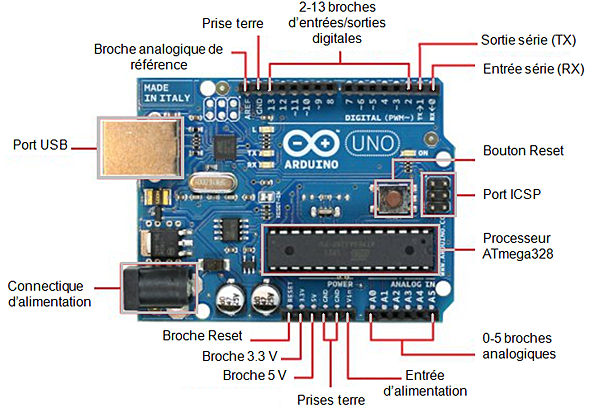
\includegraphics[width=\textwidth]{figures/Ann01}
\end{minipage}\hspace{0.2cm}\begin{minipage}{0.43\textwidth}
\captionof{figure}{Carte d'Acquisition Arduino legendée}
[tirée de \url{https://edutechwiki.unige.ch/fr/Arduino}]
\end{minipage}

Lors de l'utilisation de la carte d'acquisition, nous serons emmené à n'utiliser que la prise terre qui fixera un point du circuit à \SI{0}{\volt} et les broches analogiques qui permettra l'acquisition du potentiel en différents points du circuit.

\faWarning ~ La carte Arduino n'accepte que des potentiels inclus dans l'intervalle 0-\SI{5}{\volt}.

\subsection{Schéma du dispositif d'acquisition}

\subsection{Protocole de mise en route de l'acquisition à l'aide d'une carte Arduino}
\begin{enumerate}
\item Branchez la carte Arduino sur votre ordinateur via le câble USB 
\item A l'aide du gestionnaire de périphériques de l'ordinateur, déterminer le port COM utilisé par l'ARDUINO. 
\item Lancer l'application Arduino 
\item Sélectionner la carte « Arduino UNO » sur le logiciel Arduino
(Outils/Type de carte/Arduino Uno)
\item Sélectionner le port de communication (COM) utilisé par votre ordinateur pour dialoguer avec l'ARDUINO : outil/port/COM…
\item Vérifier que l'interface de dialogue entre la carte et python installé sur votre ordinateur est bien configuré :
\end{enumerate}

Outils/gérer les bibliothèques/chercher Firmata
\begin{itemize}
\item Ou bien Firmata est déjà installé passer à l'étape suivante
\item Ou bien vous ne trouvez pas Firmata dans la bibliothèque, il vous faut donc l'y installer :
Fichier/exemples/Firmata/standard Firmata ; ensuite téléverser Firmata sur la carte en cliquant sur la flèche du bandeau Arduino en haut à gauche.
\end{itemize}

\subsection{Code python d'acquisition}

Deux codes python sont mis à votre disposition pour réaliser l'acquisition : 
\begin{enumerate}
\item \textsc{Acquisition\_singlepoint.py} qui permet de faire une unique mesure du courant et des deux tensions qui nous intéressent.
\lstinputlisting{./Arduino/Acquisition_singlepoint.py}
\item \textsc{Acquisition\_multiplepoints.py} qui permet de faire la mesure du courant et des deux tensions qui nous intéressent pendant un intervalle de temps $\Delta t$.
\lstinputlisting{./Arduino/Acquisition_multiplepoints.py}
\end{enumerate}

	




\section{Grandeurs de réaction dans les conditons standard}
\label{sec:DrH&DrS}

Dans cette annexe, on fournit les démonstrations thermodynamiques sur lesquelles vous pouvez vous appuyez pour assimiler les grandeurs de réaction mesurées en condition ambiante aux grandeurs en condition standard.

Dans le cas de l'entropie, on part de la définition de l'entropie à pression constante : 

\begin{align}
\left( \frac{\partial G}{\partial T} \right)_{P, \xi} = - S \label{eq:def_S}
\end{align}

En utilisant le théorème de Schwart et en dérivant partiellement selon $\xi$, on a : 
\begin{align}
\left( \frac{\partial \Delta_r G}{\partial T} \right)_{P, \xi} = - \Delta_r S
\end{align}

Or on sait exprimer l'enthalpie libre de réaction : 
\begin{align}
\Delta_r G = \Delta_r G^\circ (T) + RT \ln Q
\label{eq:DrG}
\end{align}

On peut dériver partiellement l'Eq. \ref{eq:DrG} par rapport à la température : 
\begin{align}
\left( \frac{\partial}{\partial T} (\Delta_r G^\circ (T) + RT \ln Q) \right)_{P, \xi} &= - \Delta_r S \\
\left( \frac{\partial}{\partial T} \Delta_r G^\circ (T)\right)_{P, \xi}  + R \ln Q   &= - \Delta_r S \\
-\Delta_r S^\circ  + R \ln Q  &= - \Delta_r S \\
\Delta_r S^\circ  - R \ln Q  &= \Delta_r S \label{eq:DrS-DrS°}
\end{align}
L'Eq. \ref{eq:DrS-DrS°} permet de lier l'entropie de réaction à la grandeur équivalente en condition standard

Pour ce qui est l'enthalpie, il faut utiliser une astuce en partant de la définition de G : 
\begin{align}
G &= H - T S \\
G &= H + \left( \frac{\partial G}{\partial T} \right)_{P, \xi} T \quad \text{en utilisant l'Eq.}\ref{eq:def_S} \\
\frac{G}{T^2} &= \frac{H}{T^2} + \frac{1}{T} \left( \frac{\partial G}{\partial T} \right)_{P, \xi} \\
- \frac{G}{T^2} + \frac{1}{T} \left( \frac{\partial G}{\partial T} \right)_{P, \xi} &= - \frac{H}{T^2} \label{eq:pre_GibbsHelmholtz}
\end{align}
Dans l'Eq. \ref{eq:pre_GibbsHelmholtz}, le terme à gauche est la dérivée partielle du produit G/T par rapport à la température, soit : 
\begin{align}
\left( \frac{\partial \frac{G}{T}}{\partial T} \right)_{P, \xi} = - \frac{H}{T^2}
\end{align}
En utilisant le théorème de Schwart et en dérivant partiellement selon $\xi$, on a : 
\begin{align}
\left( \frac{\partial \frac{\Delta_r G}{T}}{\partial T} \right)_{P, \xi} = - \frac{\Delta_r H}{T^2}
\end{align}
On peut alors juste utiliser l'Eq. \ref{eq:DrG} :
\begin{align}
\left( \frac{\partial \frac{\Delta_r G^\circ}{T} + R \ln Q}{\partial T} \right)_{P, \xi} &= - \frac{\Delta_r H}{T^2} \\
\left( \frac{\partial \frac{\Delta_r G^\circ}{T}}{\partial T} \right)_{P, \xi} &\approx - \frac{\Delta_r H}{T^2} \\
- \frac{\Delta_r H^\circ}{T^2} &\approx - \frac{\Delta_r H}{T^2} \implies  \Delta_r H \approx \Delta_r H^\circ \label{eq:DrH-DrH°}
\end{align}
L'Eq. \ref{eq:DrH-DrH°} montre que l'enthalpie de réaction s'assimile assez bien à l'enthalpie standard de réaction.

\newpage

\begin{center}
\gradetable
\end{center}

\end{document}